\chapter{Conclusion\label{cha:chapter8}}

As is evidenced by Figure 7.1 in 2016 ``blockchain'' is undergoing an intense period of inflated expectations. 
That being the case there \textit{are} indeed practical use cases for this technology dispite the rampant over-speculation.
In this chapter we illustrate this from the perspective of industry, with application to the concept of the ``industrial data space''. 

John Henry is an American folk hero who worked as a ``steel-driving man'', hammering steel to blast away centuries-old rock in the construction of that big iron needle stitching the country together - the US railway system. Legend has it that John Henry's prowess as a steel-driver was measured in a race against a steam-powered hammer, a race he won, only to die in a pyrrhic victory with his hammer in his hand while his heart gave out from stress.
The battle for pre-eminence in the race to deliver the steam hammers of tomorrow is a tale that dates back longer than that of the Mechanical Turk. 
As more and more complicated tasks in the human repertoire yield way to computerized automation perhaps we as a species will have more time to develop our higher cognitive abilities, such as attempting to read the minds of the companies seeking to read (and recreate) our minds!

\section{Industry Impact}

The daring knight sacrifice which shattered the meticulously planned defense kicked off a chain of events that forced a full resignation in fewer than twenty moves. With that, the title of reigning world champion of chess, one of mankind's most vigorous intellectual pursuits, was bestowed on a computer.

In 1972 the World Chess Championship in Reykjav{\'i}k pitted the American Bobby Fischer against the USSR's Boris Spassky in a landmark event of the Cold War confrontation. The fateful day in 1997 when for the first time a computer was able to defeat the incumbent world champion of chess, marked a turning point in what some have labeled a new Cold War, not between world superpowers, but between men and machines.

As there are games within games there are Cold Wars within Cold Wars. Amidst the struggle to outperform humans in the tasks traditionally associated with the highest intellectual rigour there is a struggle for leadership in the determination of who exactly it will be to develop and deploy the latest and greatest of salient machines. To the victor go the spoils and the organization that can successfully pull off these feats can expect to be handsomely rewarded.

The International Business Machines Corporation (IBM) mustered the effort to put the chess champion computer Deep Blue into action and for years they have been at the forefront of the struggle to improve the cognitive ability of machines. 
In 2011 IBM's DeepQA lab spawned Watson, the question answering computer system that trounced former human champions Brad Rutter and Ken Jennings on the quiz show \textit{Jeopardy!}.

\begin{figure}
  \centering
    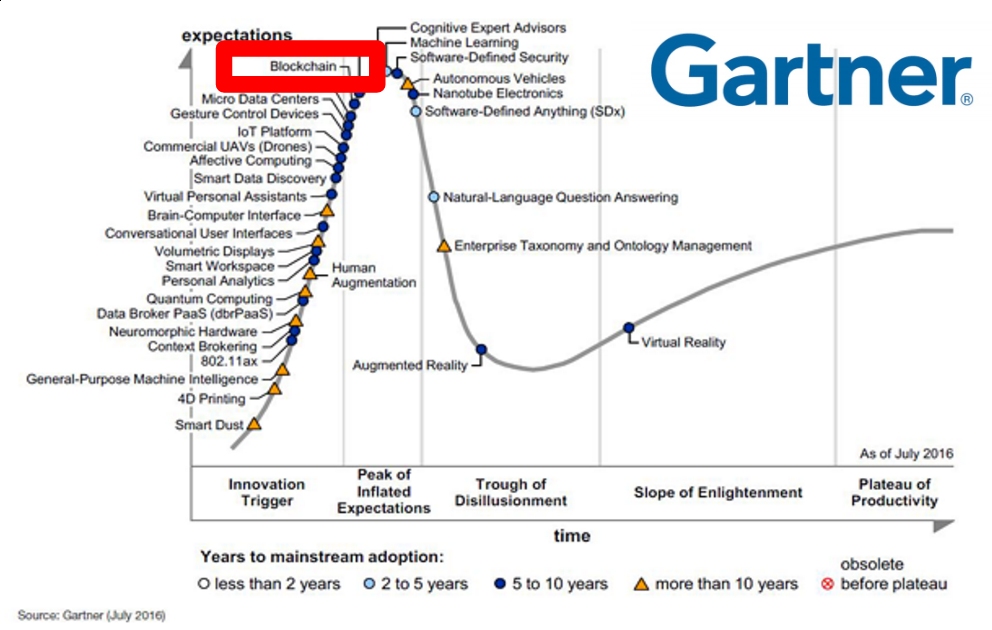
\includegraphics[width=0.75\textwidth]{go4}
  \caption{Gartner's Hype Cycle}
\end{figure}


The Cold War was an arms race. Just as the USSR's launch of Sputnik precipitated a period of frenzied turmoil for NASA, the recent success of Google's AlphaGo has sent shock waves through IBM. AlphaGo is the computer program which beat a professional human Go player, without handicaps on a full-sized 19x19 board in March 2016. As such it represents a serious challenge to IBM's storied supremacy in the race for the machine mind.

\subsection*{Can elephants dance?}

In a recent IBM symposium entitled Emerging Technologies for the Enterprise: Cognitive Computing and Blockchain. How humans and machines are forging a new age of understanding, the role of cognitive computing was described as ``systems that learn at scale, reason with purpose, and interact with humans naturally. Most important, rather than being explicitly programmed, they learn and reason from their interactions with us and from their experiences with their environment. They are made possible by advances in a number of scientific fields over the past half-century, and are different in important ways from the information systems that preceded them. Those systems have been deterministic; cognitive systems are probabilistic. They generate not just answers to numerical problems, but hypotheses, reasoned arguments, and recommendations about more complex -- and meaningful -- bodies of data''.

Fabric, IBM's contribution to the Hyperledger Project, is a Blockchain implementation with a modular architecture allowing pluggable implementations of various functions. It features powerful container technology to host any mainstream language for smart contracts development.

To date, IBMs investments in the realm of the Semantic Blockchain through the Fabric initiative have been substantial. The magnitude of IBM's moves into the space of the Semantic Blockchain portends that they anticipate this technology will play a significant role in their future. As IBM now bills themselves as a leader in the ``Cognitive Computing'' revolution, it is certain that Semantic Blockchain will play a prominent role in the next man vs. machine showdown.

\subsection*{Speak softly and carry a big stick}

The vocal advocacy of IBM in the Blockchain space stands in stark contrast to Google's almost complete silence on the subject. Prussian military theorist Carl Philipp Gottlieb von Clausewitz in his treatise \textit{On War} wrote that ``surprise plays a much greater role in strategy than in tactics'', and of course the famous Sun Tzu is remembered by the words ``when the enemy is close at hand and remains quiet, he is relying on the natural strength of his position''. 
To assume that Google is doing nothing in the Semantic Blockchain space is naive. 
Let us look forward with anticipation, and, for some, perhaps dread, to what eventually Google plans to roll out.

\section{Outlook\label{sec:outlook}}

The keen interest of large industry players in the realm of blockchain technologies has precipitated an initiative by the Linux foundation to standardize components of the so-called blockchain architecture, analogous to the way in which the World Wide Web Consortium (W3C) has endeavoured to standardize aspects of the Semantic Web. 
The effort is known as \textit{Hyperledger} and consists of a loose confederation of IT service providers interested in providing ``blockchain as a service solutions''. 
The most active members at present are IBM and to a lesser extent Intel. 
In general terms it is conceived of as a ``shared database and app engine''. 
As the fundamental exemplar of a private permissioned and consortial blockchain it will be interesting to observe how this project develops going forward. 

As noted previously Ethereum uses money as a proxy (viz. ``hack'') to solve the halting problem.
Since the cost of computation (i.e. gas) is heavily subsidized the network appears to be unsustainable.
Furthermore the community recently split in a ``hard fork'', and it appears that further partitions are imminent. 
Public commitment to migrate towards a ``proof of stake'' mining model also present potential dangers. 

The \textit{Lightning Network} is a private 2-way communication/payment channel and serves and as extension to the Bitcoin network.
This endeavour may present the ability to scale the transaction throughput of the network in a way that is acceptable to all stakeholders, thereby ensuring the long-term viability of system. 
Moreover this project is conceivably a new phase in the evolution of blockchain technology, potentially facilitating applications such as atomic cross-chain transactions.

Pegged Sidechains that utilize the Bitcoin blockchain as an infrastructure backbone upon which other coins and ideas can take shape is likewise indicative of a new direction for the future growth of the cryptocurrency ecosystem. 

\section{Concluding Discussion\label{sec:dissemination}}

With a total market capitalization in excess of \$10,000,000,000, more than 7 years of continued operation, and over 1.9 million addresses Bitcoin is the world's most successful blockchain-based cryptocurrency. 
We argue that it is the world’s \textit{only} long-term viable blockchain application to date. 
This work comprises a comprehensive programme of research undertaken into the nature of the Bitcoin protocol in an effort to assess the degree to which it's fundamental components could be applied to alternative use-cases.
The question we sought to answer was whether the data structures and incentive mechanisms that facilitate Bitcoin could be melded with semantic applications and techniques to realize concrete solutions to practical problems.
Having demonstrated this result in the affirmative we look forward to the continued growth of this burgeoning field of research. 